% Options for packages loaded elsewhere
% Options for packages loaded elsewhere
\PassOptionsToPackage{unicode}{hyperref}
\PassOptionsToPackage{hyphens}{url}
\PassOptionsToPackage{dvipsnames,svgnames,x11names}{xcolor}
%
\documentclass[
  11pt,
  a4paper,
]{article}
\usepackage{xcolor}
\usepackage{amsmath,amssymb}
\setcounter{secnumdepth}{-\maxdimen} % remove section numbering
\usepackage{iftex}
\ifPDFTeX
  \usepackage[T1]{fontenc}
  \usepackage[utf8]{inputenc}
  \usepackage{textcomp} % provide euro and other symbols
\else % if luatex or xetex
  \usepackage{unicode-math} % this also loads fontspec
  \defaultfontfeatures{Scale=MatchLowercase}
  \defaultfontfeatures[\rmfamily]{Ligatures=TeX,Scale=1}
\fi
\usepackage{lmodern}
\ifPDFTeX\else
  % xetex/luatex font selection
\fi
% Use upquote if available, for straight quotes in verbatim environments
\IfFileExists{upquote.sty}{\usepackage{upquote}}{}
\IfFileExists{microtype.sty}{% use microtype if available
  \usepackage[]{microtype}
  \UseMicrotypeSet[protrusion]{basicmath} % disable protrusion for tt fonts
}{}
\usepackage{setspace}
\makeatletter
\@ifundefined{KOMAClassName}{% if non-KOMA class
  \IfFileExists{parskip.sty}{%
    \usepackage{parskip}
  }{% else
    \setlength{\parindent}{0pt}
    \setlength{\parskip}{6pt plus 2pt minus 1pt}}
}{% if KOMA class
  \KOMAoptions{parskip=half}}
\makeatother
% Make \paragraph and \subparagraph free-standing
\makeatletter
\ifx\paragraph\undefined\else
  \let\oldparagraph\paragraph
  \renewcommand{\paragraph}{
    \@ifstar
      \xxxParagraphStar
      \xxxParagraphNoStar
  }
  \newcommand{\xxxParagraphStar}[1]{\oldparagraph*{#1}\mbox{}}
  \newcommand{\xxxParagraphNoStar}[1]{\oldparagraph{#1}\mbox{}}
\fi
\ifx\subparagraph\undefined\else
  \let\oldsubparagraph\subparagraph
  \renewcommand{\subparagraph}{
    \@ifstar
      \xxxSubParagraphStar
      \xxxSubParagraphNoStar
  }
  \newcommand{\xxxSubParagraphStar}[1]{\oldsubparagraph*{#1}\mbox{}}
  \newcommand{\xxxSubParagraphNoStar}[1]{\oldsubparagraph{#1}\mbox{}}
\fi
\makeatother


\usepackage{longtable,booktabs,array}
\usepackage{calc} % for calculating minipage widths
% Correct order of tables after \paragraph or \subparagraph
\usepackage{etoolbox}
\makeatletter
\patchcmd\longtable{\par}{\if@noskipsec\mbox{}\fi\par}{}{}
\makeatother
% Allow footnotes in longtable head/foot
\IfFileExists{footnotehyper.sty}{\usepackage{footnotehyper}}{\usepackage{footnote}}
\makesavenoteenv{longtable}
\usepackage{graphicx}
\makeatletter
\newsavebox\pandoc@box
\newcommand*\pandocbounded[1]{% scales image to fit in text height/width
  \sbox\pandoc@box{#1}%
  \Gscale@div\@tempa{\textheight}{\dimexpr\ht\pandoc@box+\dp\pandoc@box\relax}%
  \Gscale@div\@tempb{\linewidth}{\wd\pandoc@box}%
  \ifdim\@tempb\p@<\@tempa\p@\let\@tempa\@tempb\fi% select the smaller of both
  \ifdim\@tempa\p@<\p@\scalebox{\@tempa}{\usebox\pandoc@box}%
  \else\usebox{\pandoc@box}%
  \fi%
}
% Set default figure placement to htbp
\def\fps@figure{htbp}
\makeatother





\setlength{\emergencystretch}{3em} % prevent overfull lines

\providecommand{\tightlist}{%
  \setlength{\itemsep}{0pt}\setlength{\parskip}{0pt}}



 


\usepackage{fancyhdr}
\usepackage{titling}
\pagestyle{fancy}
\fancyhf{}
\fancyhead[L]{\includegraphics[height=0.5cm]{cvea-logo.png}}
\fancyhead[R]{\leftmark}
\fancyfoot[C]{\thepage}
\renewcommand{\headrulewidth}{0.4pt}
\pretitle{\begin{center}\includegraphics[width=1\textwidth]{cvea-logo.png}\\[\bigskipamount]}
\posttitle{\end{center}}
\makeatletter
\@ifpackageloaded{tcolorbox}{}{\usepackage[skins,breakable]{tcolorbox}}
\@ifpackageloaded{fontawesome5}{}{\usepackage{fontawesome5}}
\definecolor{quarto-callout-color}{HTML}{909090}
\definecolor{quarto-callout-note-color}{HTML}{0758E5}
\definecolor{quarto-callout-important-color}{HTML}{CC1914}
\definecolor{quarto-callout-warning-color}{HTML}{EB9113}
\definecolor{quarto-callout-tip-color}{HTML}{00A047}
\definecolor{quarto-callout-caution-color}{HTML}{FC5300}
\definecolor{quarto-callout-color-frame}{HTML}{acacac}
\definecolor{quarto-callout-note-color-frame}{HTML}{4582ec}
\definecolor{quarto-callout-important-color-frame}{HTML}{d9534f}
\definecolor{quarto-callout-warning-color-frame}{HTML}{f0ad4e}
\definecolor{quarto-callout-tip-color-frame}{HTML}{02b875}
\definecolor{quarto-callout-caution-color-frame}{HTML}{fd7e14}
\makeatother
\makeatletter
\@ifpackageloaded{caption}{}{\usepackage{caption}}
\AtBeginDocument{%
\ifdefined\contentsname
  \renewcommand*\contentsname{Table of contents}
\else
  \newcommand\contentsname{Table of contents}
\fi
\ifdefined\listfigurename
  \renewcommand*\listfigurename{List of Figures}
\else
  \newcommand\listfigurename{List of Figures}
\fi
\ifdefined\listtablename
  \renewcommand*\listtablename{List of Tables}
\else
  \newcommand\listtablename{List of Tables}
\fi
\ifdefined\figurename
  \renewcommand*\figurename{Figure}
\else
  \newcommand\figurename{Figure}
\fi
\ifdefined\tablename
  \renewcommand*\tablename{Table}
\else
  \newcommand\tablename{Table}
\fi
}
\@ifpackageloaded{float}{}{\usepackage{float}}
\floatstyle{ruled}
\@ifundefined{c@chapter}{\newfloat{codelisting}{h}{lop}}{\newfloat{codelisting}{h}{lop}[chapter]}
\floatname{codelisting}{Listing}
\newcommand*\listoflistings{\listof{codelisting}{List of Listings}}
\makeatother
\makeatletter
\makeatother
\makeatletter
\@ifpackageloaded{caption}{}{\usepackage{caption}}
\@ifpackageloaded{subcaption}{}{\usepackage{subcaption}}
\makeatother
\usepackage{bookmark}
\IfFileExists{xurl.sty}{\usepackage{xurl}}{} % add URL line breaks if available
\urlstyle{same}
\hypersetup{
  pdftitle={Título del Artículo en Español},
  pdfauthor={Nombre Apellido Autor 1; Nombre Apellido Autor 2},
  pdfkeywords={Palabra Clave 1, Palabra Clave 2, Palabra Clave 3},
  colorlinks=true,
  linkcolor={blue},
  filecolor={Maroon},
  citecolor={Blue},
  urlcolor={Blue},
  pdfcreator={LaTeX via pandoc}}


\title{Título del Artículo en Español}
\usepackage{etoolbox}
\makeatletter
\providecommand{\subtitle}[1]{% add subtitle to \maketitle
  \apptocmd{\@title}{\par {\large #1 \par}}{}{}
}
\makeatother
\subtitle{Subtítulo Opcional}
\author{Nombre Apellido Autor 1 \and Nombre Apellido Autor 2}
\date{2025-10-02}
\begin{document}
\maketitle
\begin{abstract}
\textbf{Resumen:} Escriba aquí el resumen estructurado en español
(máximo 250 palabras), siguiendo el orden: Antecedentes, Métodos,
Resultados y Conclusiones. \textbf{Abstract:} Write the structured
abstract in English here (maximum 250 words), following the format:
Background, Methods, Results, and Conclusions.
\end{abstract}


\setstretch{1.5}
Resumen (Ejemplo Estructurado) (Máximo 250 palabras):

\emph{(Antecedentes) La población de China e India representó
aproximadamente el 35.74\% del total mundial en 2015. Este estudio
evalúa el impacto de una variedad de indicadores demográficos,
económicos y de producción (1952-2015) en el Ingreso Nacional Bruto
(INB) de ambos países. (Métodos) Se aplicó un proceso de modelado
integral que utiliza enfoques de regresión escalonada, de regularización
(Ridge, Lasso, Elastic Net) y de rezagos distribuidos. Los resultados
teóricos se corroboraron mediante extensas pruebas de diagnóstico y una
verificación empírica de la capacidad predictiva. (Resultados) Los
hallazgos muestran que el INB en China está más influenciado por
variables como las reservas en moneda extranjera y el índice de
dependencia; mientras que, en India, las variables clave fueron la
producción de energía y la tasa de natalidad. (Conclusiones) Se sugiere
que es oportuno que China flexibilice la política universal de dos hijos
debido al valor actual por debajo de la tasa de sustitución, proyectando
un panorama sombrío para su futura población. Se pronostica un panorama
positivo para la India, dado el bajo precio futuro del petróleo.}

Abstract (Structured Example - Maximum 250 words):

\emph{(Background) In 2015, China and India's population represented
approximately 35.74\% of the total number of people living in the world.
This study assesses the impact of a wide variety of demographic,
economic, and production indicators (1952-2015) on the Gross National
Income (GNI) in China and India.(Methods) A comprehensive modeling
process with stepwise, regularization, and distributed lag regression
approaches is presented. Theoretical results were corroborated through
extensive diagnostic tests and an empirical check of the models'
predictive capacity. (Results) The findings show that GNI in China is
most influenced by variables such as reserves in foreign currency and
the dependency ratio; whereas, variables of energy production and birth
rate were generated for India. (Conclusions) It is the timing for China
to relax the universal two-child policy. A gloomy outlook for China's
future population and economy is predicted due to the current value
being below the substitution rate. Conversely, a positive outlook is
forecasted for India, given the low future price of oil---India's
primary raw material.}

\begin{tcolorbox}[enhanced jigsaw, leftrule=.75mm, titlerule=0mm, opacityback=0, breakable, colback=white, bottomtitle=1mm, left=2mm, rightrule=.15mm, colbacktitle=quarto-callout-note-color!10!white, toptitle=1mm, arc=.35mm, colframe=quarto-callout-note-color-frame, toprule=.15mm, title={Archivos Requeridos}, bottomrule=.15mm, coltitle=black, opacitybacktitle=0.6]

Para que esta plantilla funcione correctamente, asegúrese de que los
siguientes archivos estén en la misma carpeta que este documento
\texttt{.qmd}:

\begin{enumerate}
\def\labelenumi{\arabic{enumi}.}
\item
  \texttt{references.bib}: Su archivo de bibliografía.
\item
  \texttt{apa.csl}: El archivo de estilo de citación.
\item
  \textbf{REPRODUCIBILIDAD:} La Revista Venezolana de Actuariado opera
  bajo una política de datos y código abiertos. Se requiere que los
  autores carguen el código fuente completo (\texttt{.R}, \texttt{.py},
  \texttt{.jl}) y los conjuntos de datos brutos o procesados utilizados
  para generar los resultados en un repositorio público (e.g., un Saber
  UCV, GitHub, o similar) antes de la publicación, siguiendo el estándar
  de transparencia del \emph{Journal of Risk and Insurance}. La
  justificación para cualquier restricción de datos debe ser detallada y
  explícita para la revisión editorial.
\end{enumerate}

\end{tcolorbox}

\section{Introducción}\label{introducciuxf3n}

\begin{tcolorbox}[enhanced jigsaw, leftrule=.75mm, titlerule=0mm, opacityback=0, breakable, colback=white, bottomtitle=1mm, left=2mm, rightrule=.15mm, colbacktitle=quarto-callout-note-color!10!white, toptitle=1mm, arc=.35mm, colframe=quarto-callout-note-color-frame, toprule=.15mm, title=\textcolor{quarto-callout-note-color}{\faInfo}\hspace{0.5em}{Guía para el Autor: Cómo escribir una introducción eficaz}, bottomrule=.15mm, coltitle=black, opacitybacktitle=0.6]

La Introducción debe actuar como un embudo de enfoque, llevando al
lector desde el contexto general hasta el objetivo específico de su
investigación. Este es un espacio de justificación, no de síntesis
bibliográfica; la citación de la literatura seminal es vital para anclar
la discusión teórica desde las primeras frases.

\textbf{Estructura Recomendada (El Ciclo I-RL-M-R-D):}

\begin{enumerate}
\def\labelenumi{\arabic{enumi}.}
\item
  \textbf{Contexto General y Relevancia del Campo:} Comience presentando
  el campo de estudio actuarial o estadístico y su importancia macro,
  particularmente en el contexto de la economía venezolana, la
  regulación de seguros, o el mercado financiero local.
\item
  \textbf{Problema Específico (La Tensión o Controversia):} Identifique
  la controversia central, la limitación de los modelos actuales, o el
  debate teórico. Es fundamental definir qué \emph{no} se sabe sobre el
  tema (``).
\item
  \textbf{Justificación del Vacío de Conocimiento (El Porqué Aquí):}
  Articule la laguna que su estudio llenará. Dado el contexto de la
  revista, el vacío no debe ser solo metodológico, sino también de
  aplicación práctica. Debe ser explícito si el vacío es la falta de
  datos locales o la inaplicabilidad de modelos extranjeros en el
  entorno económico actual. Se requiere un acercamiento significativo al
  fenómeno para identificar qué es relevante investigar ``.
\item
  \textbf{Objetivo y Contribución:} Concluya con una declaración clara y
  concisa del objetivo. El último párrafo debe resumir de forma
  explícita la contribución novedosa de su trabajo, ya sea metodológica
  (ofreciendo un nuevo modelo), o empírica (proporcionando nuevas
  estimaciones o validaciones ).
\end{enumerate}

\end{tcolorbox}

(El cuerpo de su introducción comienza aquí\ldots)

\emph{Ejemplo: ``A pesar de que China e India han pasado por
transformaciones económicas y demográficas similares desde la segunda
mitad del siglo XX , la evolución de los indicadores demográficos y de
producción difiere significativamente debido a la intervención estatal.
Este estudio propone utilizar una amplia variedad de indicadores
demográficos y económicos para evaluar su impacto en el Ingreso Nacional
Bruto (INB) en China e India, dada la complejidad generada por las
políticas de control de natalidad\ldots{}''}

\section{Revisión Literaria}\label{revisiuxf3n-literaria}

\begin{tcolorbox}[enhanced jigsaw, leftrule=.75mm, titlerule=0mm, opacityback=0, breakable, colback=white, bottomtitle=1mm, left=2mm, rightrule=.15mm, colbacktitle=quarto-callout-note-color!10!white, toptitle=1mm, arc=.35mm, colframe=quarto-callout-note-color-frame, toprule=.15mm, title=\textcolor{quarto-callout-note-color}{\faInfo}\hspace{0.5em}{Guía para el Autor: Estructura de la Revisión Literaria Analítica
(Sección 2)}, bottomrule=.15mm, coltitle=black, opacitybacktitle=0.6]

Esta sección es obligatoria y su propósito es realizar una
\textbf{síntesis analítica y sistemática} del estado del arte,
demostrando dominio de la literatura y justificando la necesidad de la
investigación . \textbf{No debe ser un resumen cronológico o individual
de fuentes, sino una clasificación y ordenación de argumentos
temáticos.}

\textbf{Estructura para el Rigor Sistemático:}

\begin{enumerate}
\def\labelenumi{\arabic{enumi}.}
\item
  \textbf{Metodología de la Revisión:} Especifique el tipo de revisión
  realizada (ej. Revisión Sistemática, Revisión de Alcance, Revisión
  Sistematizada) y las fases seguidas (Búsqueda, Presentación de
  Resultados, Almacenamiento, Organización).
\item
  \textbf{Estrategia de Búsqueda:} Describa de forma replicable los
  términos clave de búsqueda, los operadores booleanos y los criterios
  de inclusión/exclusión. Liste las bases de datos académicas
  consultadas, priorizando las de alta confiabilidad como Scopus, Scielo
  y Redalyc, además de Google Académico ``. Se recomienda utilizar los
  códigos JEL opcionales del manuscrito como parte de la estrategia para
  identificar la literatura más relevante en Economía y Finanzas
  Actuariales (G22, C53, J11).
\item
  \textbf{Clasificación y Síntesis Analítica:}

  \begin{itemize}
  \item
    Organice el cuerpo de la sección por \textbf{temas, controversias o
    clases de modelos} (ej. ``Modelos Estocásticos de Tasa de Interés,''
    o ``Riesgo de Catástrofe en Mercados Emergentes'').
  \item
    Para la organización interna, se sugiere utilizar una \textbf{Matriz
    de Síntesis} para clasificar y comparar los diferentes argumentos
    presentados. En esta matriz (que puede ser implícita o descrita),
    coteje los atributos clave de los estudios revisados: (1) Modelos
    utilizados (e.g., Lee-Carter vs.~CBD), (2) Tipo y origen de los
    datos, y (3) Principales Conclusiones y Limitaciones.
  \item
    Identifique los referentes empíricos, los casos modelo, y las
    controversias o debates conceptuales.
  \end{itemize}
\item
  \textbf{Conclusión de la Revisión:} Finalice la RL con una sección que
  identifique las controversias o las \textbf{cuestiones que permanecen
  sin respuesta} en la literatura. Este cierre debe justificar de manera
  explícita la elección de la metodología del estudio que se detalla a
  continuación.
\end{enumerate}

\end{tcolorbox}

(El cuerpo de su Revisión Literaria en Profundidad comienza aquí\ldots)

\emph{Ejemplo: ``La modelización actuarial moderna exige técnicas de
selección de variables robustas. La literatura propone métodos de
regularización como Ridge, Lasso y Elastic Net para mitigar problemas de
multicolinealidad , ofreciendo alternativas superiores a la selección
secuencial tradicional. Específicamente, el método Lasso es valorado por
su capacidad de contracción (shrinkage) que realiza una selección
continua de variables, forzando coeficientes a cero para simplificar el
modelo\ldots{}''}

\section{Métodos}\label{muxe9todos}

\begin{tcolorbox}[enhanced jigsaw, leftrule=.75mm, titlerule=0mm, opacityback=0, breakable, colback=white, bottomtitle=1mm, left=2mm, rightrule=.15mm, colbacktitle=quarto-callout-note-color!10!white, toptitle=1mm, arc=.35mm, colframe=quarto-callout-note-color-frame, toprule=.15mm, title=\textcolor{quarto-callout-note-color}{\faInfo}\hspace{0.5em}{Guía para el Autor: El Rigor Actuarial y la Replicabilidad del Código
(Sección 3)}, bottomrule=.15mm, coltitle=black, opacitybacktitle=0.6]

Esta sección es la ``receta'' completa del estudio. Debe ser tan
detallada que otro investigador, con el mismo código y datos, pueda
replicar su estudio y confirmar los hallazgos ``. En las ciencias
actuariales, esto implica un alto nivel de transparencia computacional.

\textbf{Requisitos Detallados:}

\begin{enumerate}
\def\labelenumi{\arabic{enumi}.}
\item
  \textbf{Diseño del Estudio y Estrategia Empírica:} Defina si el
  trabajo es primordialmente metodológico (proponiendo o refinando
  técnicas) o empírico (aplicando técnicas a datos). Si el trabajo es
  empírico, justifique la \textbf{estrategia de identificación} empleada
  para establecer relaciones causales o si los hallazgos son
  fundamentalmente descriptivos. La validez de los métodos debe ser
  apropiada para responder la pregunta de investigación.
\item
  \textbf{Fuentes de Datos y Muestras:} Especifique la procedencia de
  los datos, la temporalidad, y el tamaño de la muestra. Describa
  detalladamente los procesos de preprocesamiento, normalización o
  ajuste de datos, indicando las herramientas utilizadas.
\item
  \textbf{Modelización y Procedimientos:}

  \begin{itemize}
  \item
    Describa los modelos matemáticos y estadísticos aplicados,
    incluyendo la justificación para su selección basada en la Revisión
    Literaria (Sección 2).
  \item
    Detalle los parámetros, supuestos, métodos de calibración (e.g.,
    Método de Sustitución, ANOVA para estudios R\&R) y los
    procedimientos de validación fuera de muestra.
  \end{itemize}
\item
  \textbf{Formato de Ecuaciones:} Las ecuaciones deben escribirse
  utilizando la sintaxis de LaTeX/Quarto (dentro de \texttt{\$\ \$} o
  \texttt{\$\$\ \$\$}), y deben numerarse consecutivamente a lo largo de
  todo el documento. Las referencias textuales deben ser claras, como
  ``la ecuación (3) indica\ldots{}'' ``.
\item
  \textbf{Entorno Computacional y Código Fuente:} Esta sección debe
  listar el software, el lenguaje de programación (R, Python, Julia,
  etc.) y las versiones exactas de todos los paquetes o librerías
  críticas utilizadas. El código fuente completo y los datos deben estar
  disponibles en un repositorio público, tal como se detalla en la
  política de reproducibilidad al inicio del documento ``.
\end{enumerate}

\end{tcolorbox}

(El cuerpo de su sección de Métodos comienza aquí\ldots)

\emph{Ejemplo: ``Para la validación de los modelos de regresión lineal,
se implementó el método Global Validation of Linear Model Assumptions
propuesto por Peña y Slate (2006) , que evalúa las dimensiones de
Asimetría (Skewness), Curtosis (Kurtosis), Linealidad y
Heteroscedasticidad. Este enfoque se complementó con pruebas específicas
para las series de tiempo, como las pruebas de Box-Pierce y Ljung-Box
para la autocorrelación de los residuos , y la prueba de Breusch-Pagan
(1979) para heteroscedasticidad\ldots{}''}

\section{Resultados}\label{resultados}

\begin{tcolorbox}[enhanced jigsaw, leftrule=.75mm, titlerule=0mm, opacityback=0, breakable, colback=white, bottomtitle=1mm, left=2mm, rightrule=.15mm, colbacktitle=quarto-callout-note-color!10!white, toptitle=1mm, arc=.35mm, colframe=quarto-callout-note-color-frame, toprule=.15mm, title=\textcolor{quarto-callout-note-color}{\faInfo}\hspace{0.5em}{Guía para el Autor: Presentación Objetiva y Coherencia Visual
Reproducible (Sección 4)}, bottomrule=.15mm, coltitle=black, opacitybacktitle=0.6]

En esta sección, se presentan los hallazgos de la investigación de
manera objetiva, siguiendo la secuencia de los pasos metodológicos.
\textbf{No es recomendable interpretar, discutir las implicaciones de
los resultados, o compararlos con la literatura aquí; esta actividad se
reserva para la Discusión (Sección 5) ``}.

\textbf{Estándares de Presentación:}

\begin{enumerate}
\def\labelenumi{\arabic{enumi}.}
\item
  \textbf{Narrativa Secuencial:} Guíe al lector a través de los
  resultados en el mismo orden en que fueron descritos los
  procedimientos en la Sección 3.
\item
  \textbf{Visualización de Datos:} Utilice las capacidades de Quarto
  para la generación de gráficos de alta calidad a partir de los bloques
  de código (R con \texttt{ggplot2}, Python con \texttt{seaborn}, Julia
  con \texttt{Plots.jl}, etc.).

  \begin{itemize}
  \item
    \textbf{Leyendas Completas (Captions):} Cada Figura y Tabla debe
    tener una leyenda descriptiva y completa (\texttt{fig-cap}) que se
    explique por sí misma, sin requerir la lectura del texto adyacente
    ``.
  \item
    \textbf{Referenciación Cruzada:} Utilice la funcionalidad de Quarto
    para referenciar automáticamente todas las Figuras y Tablas en el
    texto (ej. ``La tendencia se ilustra en la Figura @fig-r-dist'').
  \end{itemize}
\item
  \textbf{Tablas y Números:} Las tablas deben ser concisas. Las columnas
  deben estar clara y descriptivamente etiquetadas ``. Solo presente los
  estadísticos y cifras esenciales que contribuyen a responder la
  pregunta de investigación.
\item
  \textbf{Trazabilidad del Código:} Asegúrese de que todos los bloques
  de código que generaron los resultados visuales y numéricos estén
  presentes en el archivo \texttt{.qmd} (aunque se puede usar
  \texttt{echo:\ false} para ocultar el código en el documento final,
  como se ve en los ejemplos de la plantilla), garantizando la
  trazabilidad y la revisabilidad.
\end{enumerate}

\end{tcolorbox}

\emph{Ejemplo: ``El análisis de multicolinealidad de los modelos de
regresión secuencial seleccionados (Tabla 9) muestra que la
transformación de la tasa de crecimiento, primera diferencia (Gro Diff)
para China, fue la única que superó todas las pruebas de diagnóstico
global (Tabla 10). Específicamente, esta transformación se centró en las
variables Gasto Gubernamental (GV.EX) y Producción de Energía (EN.PR),
confirmando su relevancia estructural\ldots{}''}

\subsection*{la Programación en la Modelización Cuantitativa
Moderna}\label{la-programaciuxf3n-en-la-modelizaciuxf3n-cuantitativa-moderna}
\addcontentsline{toc}{subsection}{la Programación en la Modelización
Cuantitativa Moderna}

El análisis de datos en el siglo XXI, particularmente en campos que
exigen alta precisión como la econometría avanzada, la ciencia de datos
y el modelado actuarial, requiere herramientas de programación que
satisfagan un complejo conjunto de demandas. La investigación
cuantitativa moderna requiere entornos de cómputo que armonicen tres
objetivos a menudo ortogonales: potencia estadística (para la
inferencia), velocidad de ejecución (para la simulación y el cálculo
intensivo) y capacidad de despliegue industrial (para la producción a
escala).

R, Python y Julia se han consolidado como los principales lenguajes de
programación en el ámbito de la computación científica, cada uno
enfocado en resolver uno o más aspectos de este desafío. La elección de
la plataforma adecuada no es trivial, ya que el analista debe
inherentemente ponderar qué objetivo ---el rigor estadístico, la
facilidad de producción o el rendimiento puro--- es el más crítico para
el éxito del proyecto. Esta tensión en la optimización es la base del
dilema tecnológico en el sector cuantitativo.

A continuación una breve descripción y una evaluación comparativa de
estos tres lenguajes.

\subsection*{R: La Cuna de la Estadística
Moderna}\label{r-la-cuna-de-la-estaduxedstica-moderna}
\addcontentsline{toc}{subsection}{R: La Cuna de la Estadística Moderna}

R es el heredero de una tradición de décadas en el análisis de datos. Es
una implementación de código abierto del lenguaje S, desarrollado
originalmente en Bell Laboratories por John Chambers y sus colegas. Los
principales creadores de R son Ross Ihaka y Robert Gentleman.

El lenguaje se integró oficialmente en el Proyecto GNU en 1997, marcando
un hito con la Versión 0.60 el 5 de diciembre de ese año. Desde su
concepción, R ha sido un entorno integral centrado en la computación
estadística y gráfica, ofreciendo una amplia variedad de técnicas de
modelado (lineal, no lineal, series de tiempo, clasificación) y una
suite de operadores para el cálculo en arreglos y matrices.

El ecosistema principal de R, el CRAN (Comprehensive R Archive Network),
es notable no solo por el volumen de sus paquetes, sino por su rigor
académico. La comunidad exige documentación detallada y, a menudo, la
funcionalidad de los paquetes está respaldada por publicaciones
revisadas por pares en revistas especializadas, como el Journal of
Statistical Software. Esta exigencia de documentación y validación
confiere a R una credibilidad crucial para la inferencia de alto riesgo
y explica por qué los libros de texto actuariales y estadísticos
continúan utilizando R de forma extensiva.

Por ejemplo en el lenguaje R, tiene paquetes como \texttt{ggplot2}, que
es una herramienta poderosa para la visualización de datos estadísticos.

La Figura Figure~\ref{fig-r-dist} muestra una comparación de la
distribución de la masa corporal entre tres especies de pingüinos,
combinando curvas de densidad con los puntos de datos reales.

\begin{figure}

\centering{

\pandocbounded{\includegraphics[keepaspectratio]{jfwm_template_raw_files/figure-pdf/fig-r-dist-1.pdf}}

}

\caption{\label{fig-r-dist}Gráfico de lluvia (raincloud plot) mostrando
la distribución de la masa corporal (g) para tres especies de pingüinos.
Combina una curva de densidad con puntos de datos individuales para una
visualización más completa.}

\end{figure}%

\begin{figure}

\centering{

\pandocbounded{\includegraphics[keepaspectratio]{jfwm_template_raw_files/figure-pdf/fig-r-dist2-1.pdf}}

}

\caption{\label{fig-r-dist2}Análisis de regresión facetado que muestra
la relación entre la longitud del pico y la longitud de la aleta para
tres especies de pingüinos, con líneas de regresión lineal y sus
intervalos de confianza.}

\end{figure}%

\subsection*{Python: El Lenguaje de Propósito
General}\label{python-el-lenguaje-de-propuxf3sito-general}
\addcontentsline{toc}{subsection}{Python: El Lenguaje de Propósito
General}

Python fue concebido por Guido van Rossum, con su publicación inicial en
1991. Su diseño se centró en la legibilidad y una sintaxis simple,
ofreciendo una curva de aprendizaje baja que ha contribuido a su
adopción masiva.

Originalmente un lenguaje de propósito general, la expansión de Python
en el dominio de la ciencia de datos fue impulsada por la creación de
librerías de alto rendimiento, como NumPy y Pandas, que actúan como
wrappers para delegar el cómputo intensivo (cálculos matriciales,
manipulación de datos) a código escrito en C o Fortran, mitigando así la
lentitud del código Python puro.

Su repositorio central, PyPI (Python Package Index), es el más grande
del mundo, lo que es indicativo de su vasto alcance en tareas que van
desde la programación de sistemas operativos y desarrollo web hasta la
infraestructura de Machine Learning. La filosofía de sus paqueterías
tiende a favorecer herramientas grandes y monolíticas, cubriendo amplias
áreas funcionales (ej. un paquete grande para todo el flujo de ML), lo
que contrasta con el enfoque modular de Julia y R.

Python, con librerías como \texttt{seaborn}, es ideal para exploraciones
visuales de datos. La Figura Figure~\ref{fig-py-pairplot} muestra las
relaciones bivariadas y distribuciones univariadas de las medidas
biométricas de los pingüinos, coloreadas por especie.

\begin{figure}

\centering{

\pandocbounded{\includegraphics[keepaspectratio]{jfwm_template_raw_files/figure-pdf/fig-py-pairplot-1.pdf}}

}

\caption{\label{fig-py-pairplot}Gráfico de pares (pairplot) de las
variables numéricas del conjunto de datos \texttt{penguins}, generado
con Seaborn en Python. La diagonal muestra la distribución de cada
variable por especie, y los otros paneles muestran las relaciones
bivariadas.}

\end{figure}%

\begin{figure}

\centering{

\pandocbounded{\includegraphics[keepaspectratio]{jfwm_template_raw_files/figure-pdf/fig-py-pairplot2-3.pdf}}

}

\caption{\label{fig-py-pairplot2}Gráfico de contorno de densidad 2D
(Kernel Density Estimate) que muestra la relación entre la longitud y la
profundidad del pico para cada especie de pingüino. Las áreas más
oscuras indican una mayor concentración de datos.}

\end{figure}%

\subsection*{Julia: Abordando el ``Problema del Lenguaje
Dual''}\label{julia-abordando-el-problema-del-lenguaje-dual}
\addcontentsline{toc}{subsection}{Julia: Abordando el ``Problema del
Lenguaje Dual''}

Julia es el lenguaje más reciente de la tríada, creado por Jeff
Bezanson, Stefan Karpinski, Viral B. Shah y Alan Edelman, entre otros, y
su versión de estabilidad (1.0) se lanzó en 2018. Julia fue diseñado
específicamente para la computación científica de alto rendimiento.

La misión central de Julia es resolver el \textbf{``Problema del
Lenguaje Dual''}. Este problema se manifiesta cuando un investigador
prototipa un algoritmo en un lenguaje de alto nivel (fácil de codificar,
como Python o R), pero luego se ve obligado a reescribir ese código en
un lenguaje de bajo nivel (rápido, como C++) para lograr la velocidad
necesaria en entornos de producción.

Julia busca combinar la facilidad de escritura del código de alto nivel
con la velocidad de ejecución de los lenguajes de bajo nivel, utilizando
una arquitectura innovadora, incluyendo un compilador
\emph{Just-in-Time} (JIT). Esto permite que el desarrollo del algoritmo
y la implementación en producción se realicen con un único código base
rápido.

El ecosistema de Julia, General Registry, promueve paquetes que son, en
promedio, 4.4 veces más pequeños que los paquetes medianos de Python,
fomentando la composición de bibliotecas altamente especializadas a
través de su característica clave, el \emph{Multiple Dispatch}.

Se pordría decir entonces que Julia es un lenguaje de alto rendimiento
excelente para la computación científica intensiva. A continuación, se
muestra un gráfico de superficie 3D para demostrar su uso en
visualización avanzada.

\begin{tcolorbox}[enhanced jigsaw, leftrule=.75mm, titlerule=0mm, opacityback=0, breakable, colback=white, bottomtitle=1mm, left=2mm, rightrule=.15mm, colbacktitle=quarto-callout-tip-color!10!white, toptitle=1mm, arc=.35mm, colframe=quarto-callout-tip-color-frame, toprule=.15mm, title=\textcolor{quarto-callout-tip-color}{\faLightbulb}\hspace{0.5em}{Nota sobre la Ejecución de Julia}, bottomrule=.15mm, coltitle=black, opacitybacktitle=0.6]

El siguiente bloque de código de Julia se ejecuta gracias a un bloque de
configuración de R previo que prepara el entorno de Julia antes de su
uso.

\end{tcolorbox}

\begin{verbatim}
-10.0:0.5:10.0
\end{verbatim}

\begin{verbatim}
-10.0:0.5:10.0
\end{verbatim}

\begin{verbatim}
f (generic function with 1 method)
\end{verbatim}

\begin{figure}

\centering{

\pandocbounded{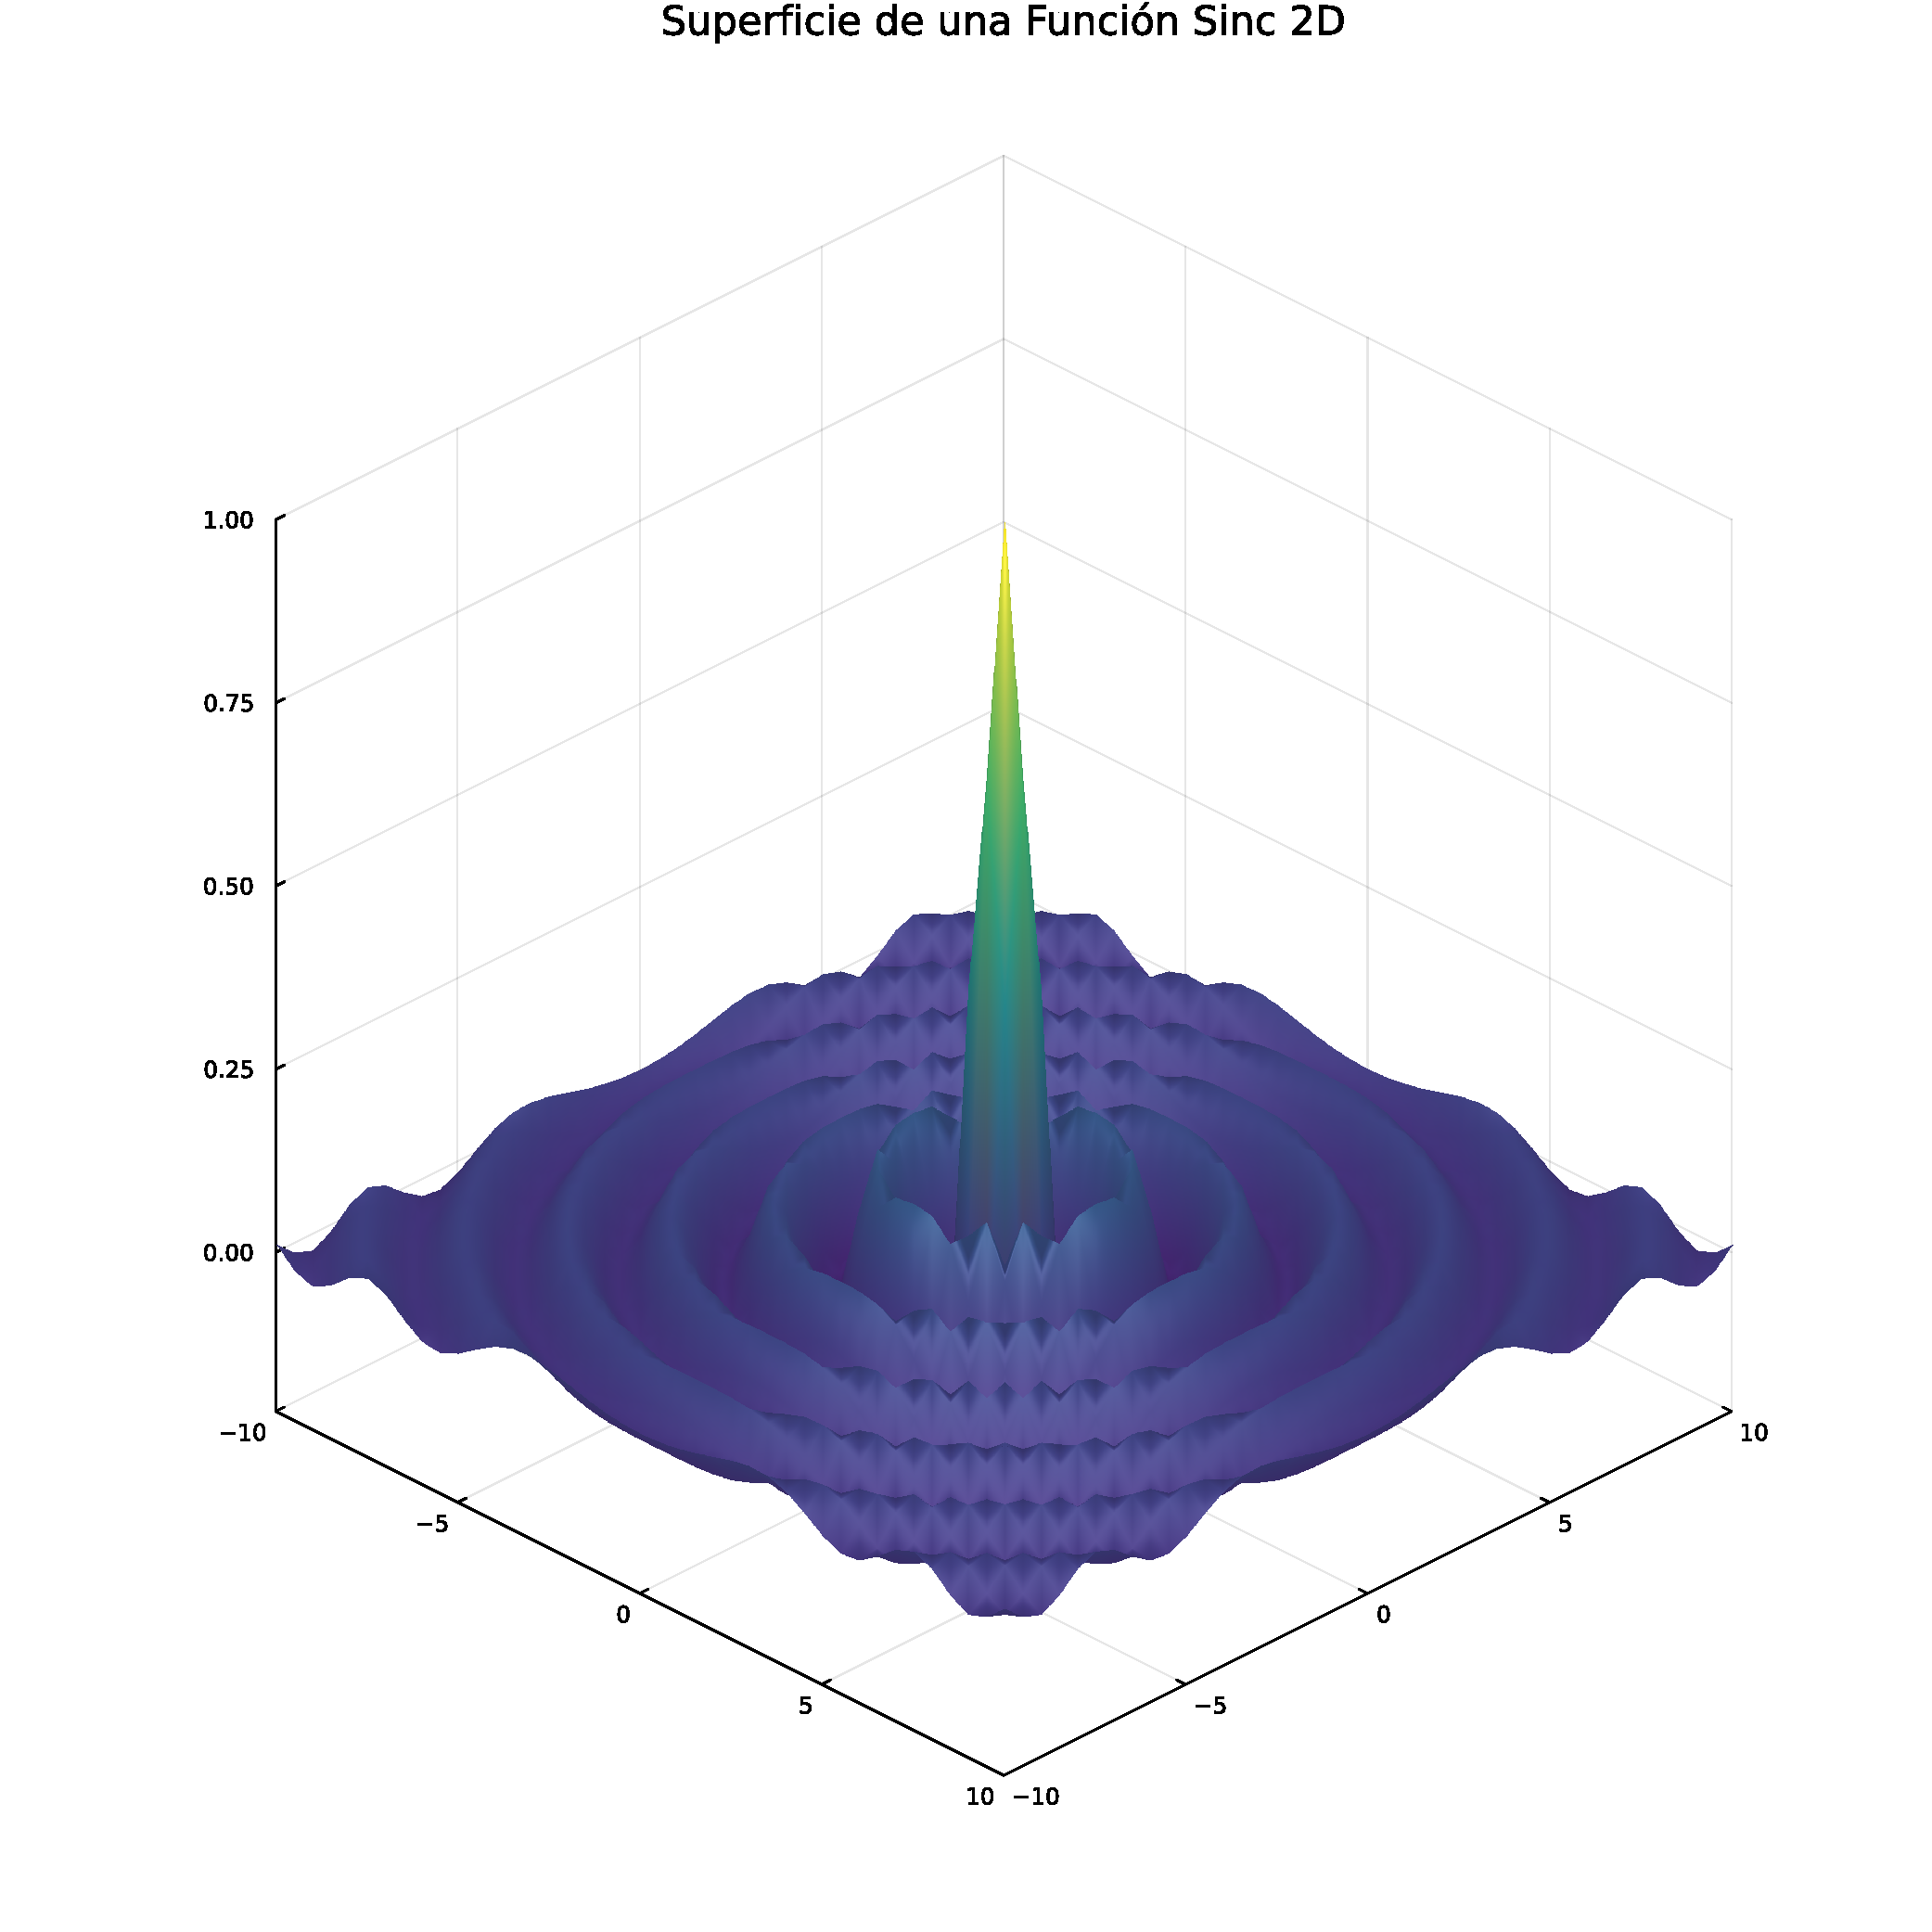
\includegraphics[keepaspectratio]{jfwm_template_raw_files/figure-pdf/fig-julia-surface-J1.pdf}}

}

\caption{\label{fig-julia-surface}Gráfico de superficie 3D de la función
f(x, y) = sinc(sqrt(x\^{}2 + y\^{}2)) generado con Plots.jl en Julia.}

\end{figure}%

El siguiente bloque de código de Julia se ejecuta gracias a un bloque de
configuración de R previo que prepara el entorno de Julia antes de su
uso.

\begin{verbatim}
(0.0, 50.0)
\end{verbatim}

\begin{figure}

\centering{

\pandocbounded{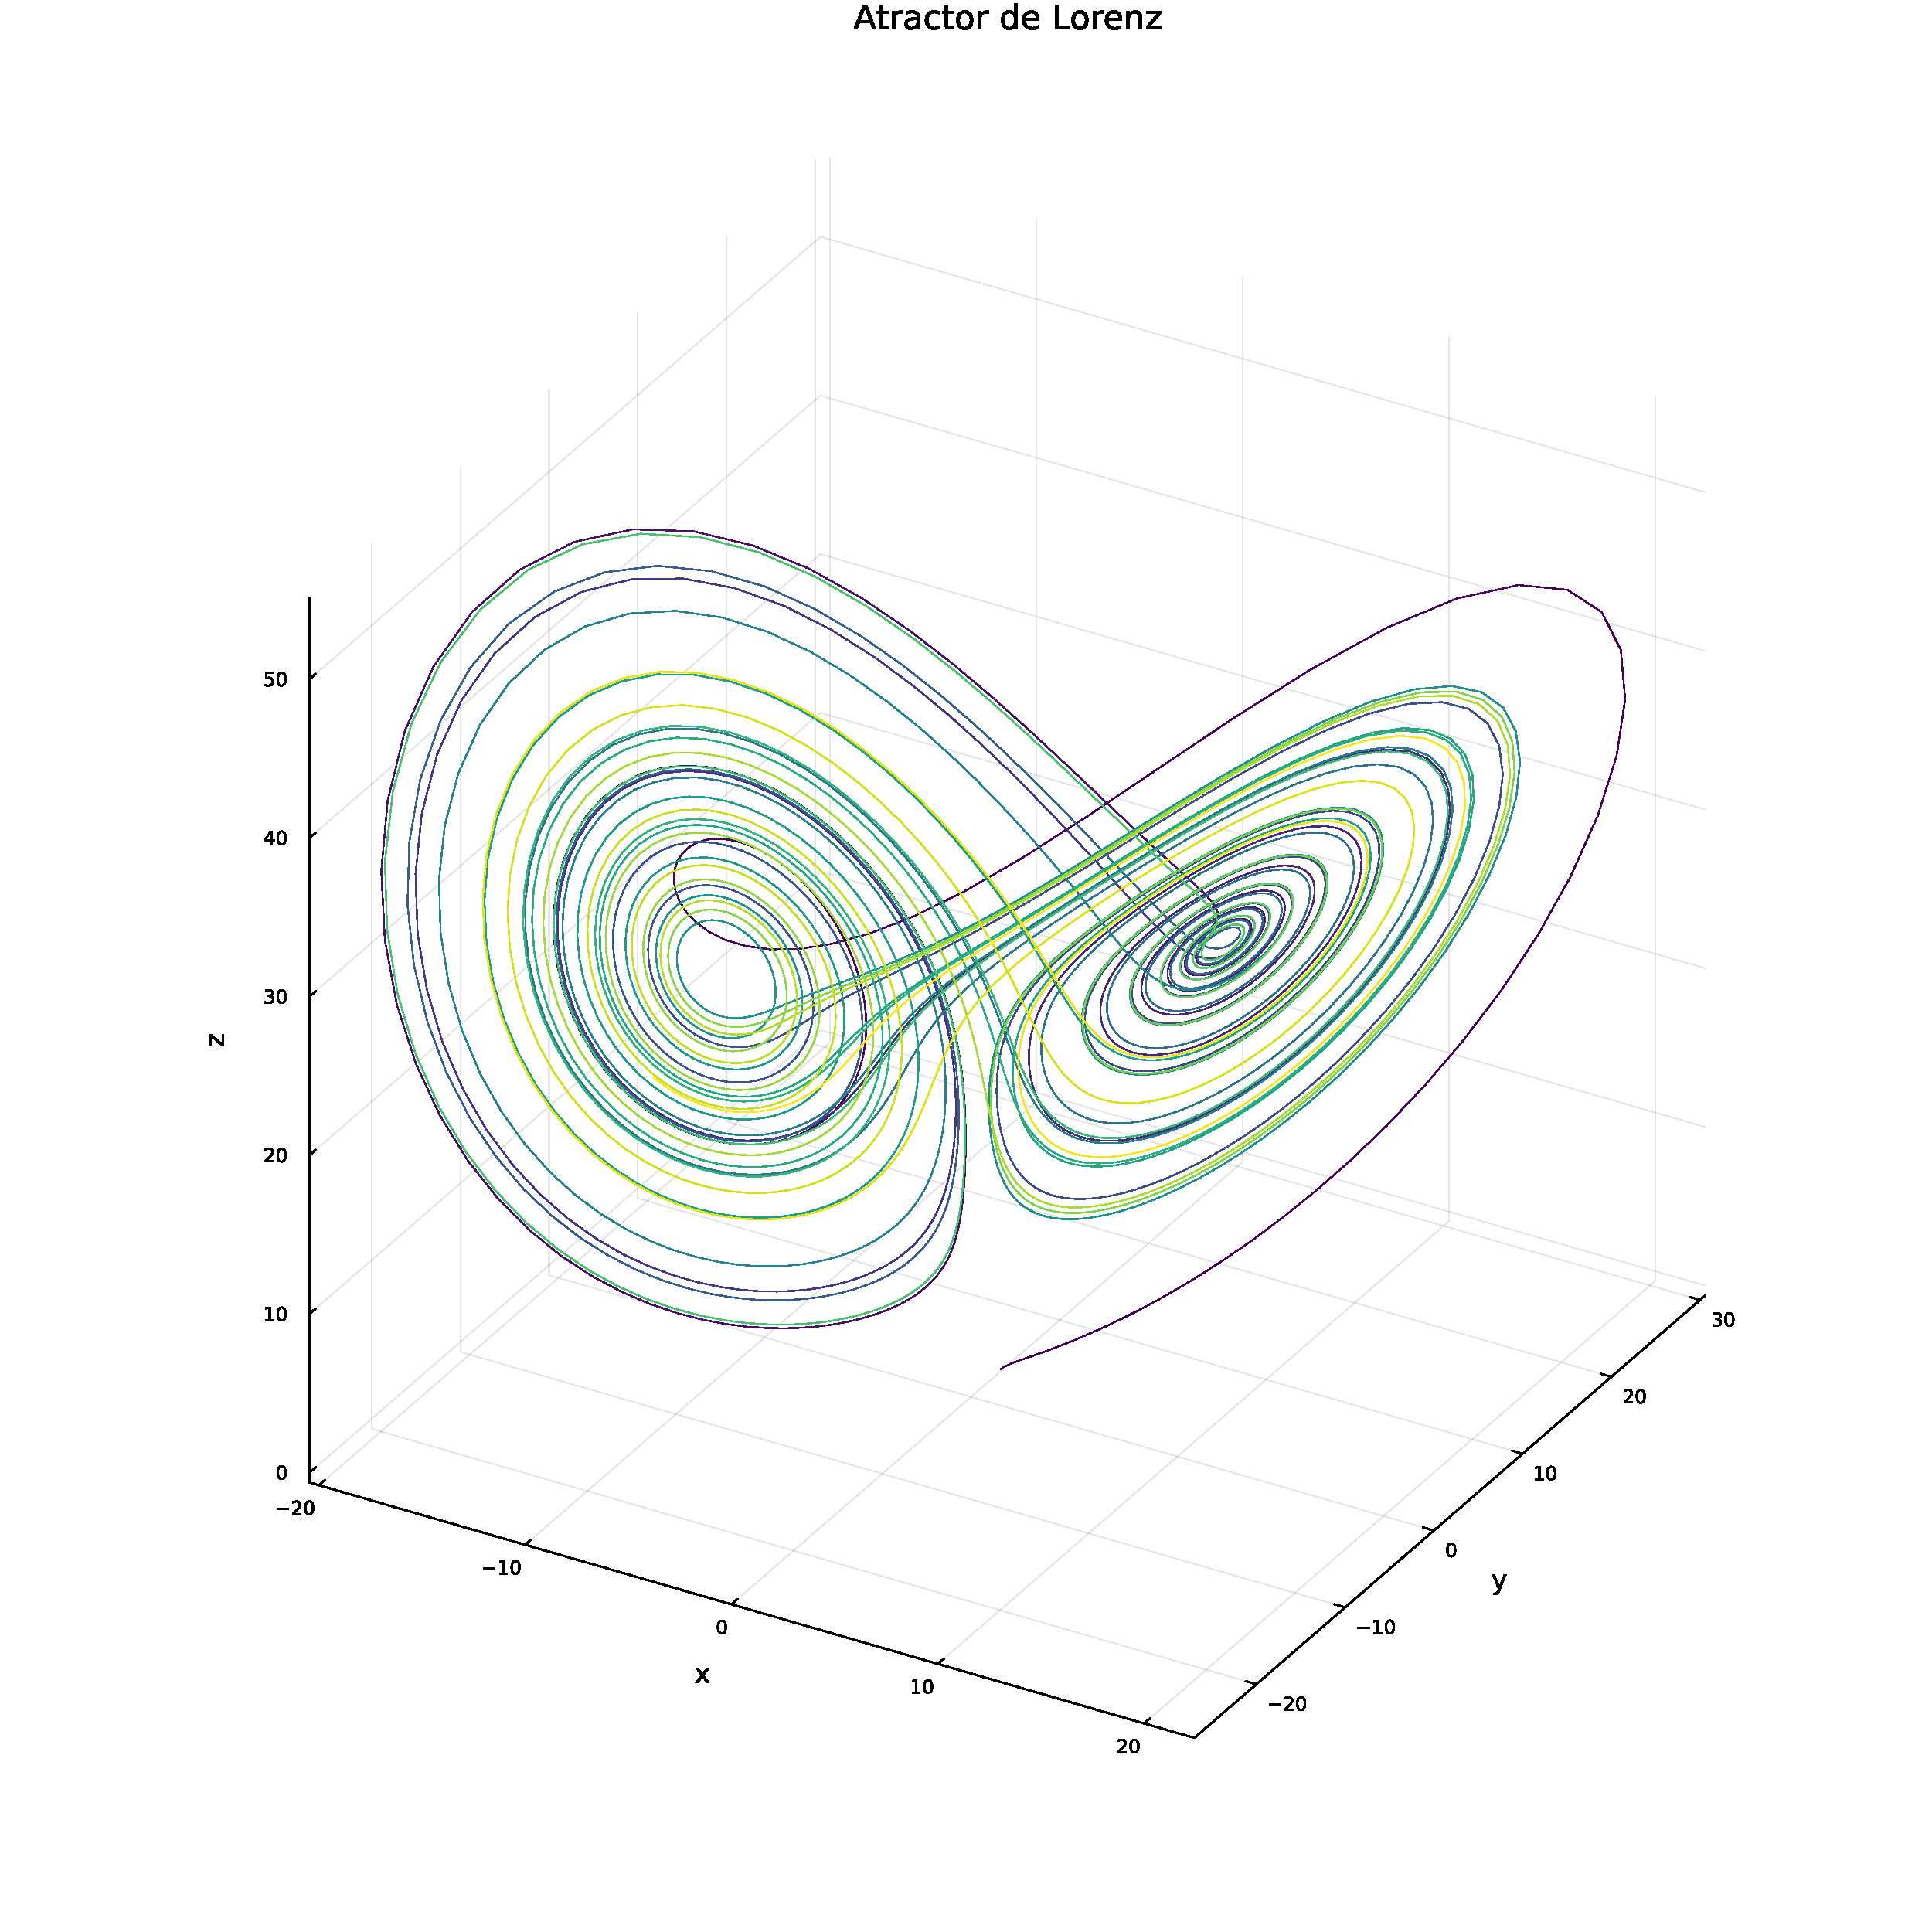
\includegraphics[keepaspectratio]{jfwm_template_raw_files/figure-pdf/fig-julia-lorenz-J1.pdf}}

}

\caption{\label{fig-julia-lorenz}Visualización del Atractor de Lorenz,
un sistema dinámico caótico, generado con Plots.jl en Julia. Este tipo
de gráfico demuestra la capacidad de Julia para la simulación numérica y
la visualización 3D.}

\end{figure}%

\subsection*{Síntesis de Fortalezas y
Debilidades}\label{suxedntesis-de-fortalezas-y-debilidades}
\addcontentsline{toc}{subsection}{Síntesis de Fortalezas y Debilidades}

Los lenguajes R, Python y Julia han cimentado su lugar en la computación
científica al minimizar diferentes fricciones en el flujo de trabajo del
analista:

\begin{itemize}
\item
  Recomendación para la Inferencia y Validación (Elegir R): R es la
  opción superior cuando el foco es el modelado estadístico riguroso y
  la necesidad de generar documentación y gráficos de calidad de
  publicación. La madurez de su ecosistema CRAN proporciona un nivel de
  confianza y validación metodológica inigualable en la estadística
  clásica.
\item
  Recomendación para la Producción y Escalabilidad (Elegir Python):
  Python debe ser seleccionado cuando el objetivo principal es la
  integración de modelos en pipelines de software empresariales, la
  aplicación de Deep Learning o la necesidad de contar con una gran
  reserva de talento y una infraestructura de despliegue madura. Su rol
  como lenguaje de propósito general lo convierte en el estándar para la
  producción industrial.
\item
  Recomendación para la Simulación de Alto Rendimiento (Elegir Julia):
  Julia es la herramienta esencial cuando el cuello de botella del
  proyecto es la velocidad de ejecución. Es ideal para la simulación
  numérica de gran escala, la optimización y el modelado actuarial
  cuantitativo que exige un rendimiento extremo. Las organizaciones que
  buscan reducir drásticamente los tiempos de cálculo de capital de
  riesgo o implementar nuevos modelos dinámicos encontrarán en Julia el
  motor de Cómputo de Alto Rendimiento (HPC) más eficiente disponible
  sin la necesidad de reescribir la lógica en C++.
\end{itemize}

La competencia en el análisis cuantitativo moderno raramente se resuelve
con la elección de un solo lenguaje. La capacidad de Julia para
interactuar con librerías de R y Python subraya la importancia de la
interoperabilidad. Los analistas cuantitativos más efectivos son
aquellos que pueden navegar fluidamente entre al menos dos de estas
plataformas, utilizando R para el análisis exploratorio y la
visualización final, Python para la integración de Big Data y ML, y
Julia para la simulación de riesgo intensiva en cómputo.

\section{Discusión y Conclusiones}\label{discusiuxf3n-y-conclusiones}

\begin{tcolorbox}[enhanced jigsaw, leftrule=.75mm, titlerule=0mm, opacityback=0, breakable, colback=white, bottomtitle=1mm, left=2mm, rightrule=.15mm, colbacktitle=quarto-callout-tip-color!10!white, toptitle=1mm, arc=.35mm, colframe=quarto-callout-tip-color-frame, toprule=.15mm, title=\textcolor{quarto-callout-tip-color}{\faLightbulb}\hspace{0.5em}{Guía para el Autor: Síntesis, Contraste y Proyección (Sección 5)}, bottomrule=.15mm, coltitle=black, opacitybacktitle=0.6]

Esta sección es el componente interpretativo de su investigación. Su
objetivo es ir más allá de los datos brutos (Sección 4) y explicar su
significado, contrastándolos rigurosamente con el corpus teórico
establecido en la Revisión Literaria (Sección 2).

\textbf{Estructura Crítica (El Diálogo con la RL):}

\begin{enumerate}
\def\labelenumi{\arabic{enumi}.}
\item
  \textbf{Interpretación y Respuesta a la Pregunta:} La Discusión debe
  comenzar abordando directamente la pregunta de investigación y luego
  interpretar los hallazgos más relevantes. Se deben evitar frases que
  simplemente repitan los resultados; el enfoque debe ser el
  \emph{porqué} de esos resultados.
\item
  \textbf{Diálogo con la Literatura (Contraste):} Compare sus resultados
  directamente con los trabajos clave identificados y analizados en la
  Sección 2 (Revisión Literaria).

  \begin{itemize}
  \item
    \textbf{Contraste Explícito:} ¿Por qué su modelo o aplicación
    divergió de los estudios previos? ¿Sus resultados confirman las
    tendencias globales o revelan una dinámica única del mercado
    venezolano?
  \item
    \textbf{Resolución de Controversias:} Si la Revisión Literaria
    identificó un debate teórico o una controversia, esta sección es
    donde usted expone cómo sus resultados contribuyen a resolverla o a
    redefinirla.
  \item
    \textbf{Soporte Bibliográfico:} Toda afirmación interpretativa,
    especialmente si es una conclusión importante o una comparación,
    debe estar apoyada por citas bibliográficas.
  \end{itemize}
\item
  \textbf{Limitaciones y Autocrítica:} Discuta honestamente las
  debilidades metodológicas, las restricciones de datos, o los supuestos
  que podrían afectar la generalizabilidad de los resultados.
\item
  \textbf{Implicaciones y Futuras Direcciones:} Explique las
  implicaciones prácticas de sus hallazgos para la industria, la
  academia o la política regulatoria. Proponga líneas claras de
  investigación futura que surjan de las limitaciones o de los
  resultados inesperados.
\item
  \textbf{Conclusión Final:} Concluya con un párrafo que sintetice la
  contribución principal y el impacto de su trabajo, asegurando que esta
  contribución esté claramente enmarcada dentro de la literatura
  actuarial\textbf{.}
\end{enumerate}

\end{tcolorbox}

(El cuerpo de su sección de Discusión comienza aquí\ldots)

\emph{Ejemplo: ``Los resultados confirman que el Gasto Gubernamental
(GV.EX) es un factor clave en China debido a la planificación económica
quinquenal del estado. Sin embargo, la persistencia de las políticas de
control de natalidad, reflejadas en el ratio de dependencia, podría
generar efectos adversos a largo plazo en el INB, sugiriendo una
reevaluación de las restricciones demográficas para evitar una situación
similar a la de Japón, con un alto ratio de dependencia en la
vejez\ldots{}''}

\section*{Agradecimientos}\label{agradecimientos}
\addcontentsline{toc}{section}{Agradecimientos}

Sección opcional para agradecer a personas o instituciones que
contribuyeron al trabajo pero no cumplen los criterios de autoría (ej.
financiamiento, revisión de estilo, etc.).

\section*{Referencias}\label{referencias}
\addcontentsline{toc}{section}{Referencias}

La lista de referencias se generará automáticamente aquí a partir del
archivo \texttt{references.bib} y las citas usadas en el texto. No es
necesario escribir nada en esta sección.

\begin{tcolorbox}[enhanced jigsaw, leftrule=.75mm, titlerule=0mm, opacityback=0, breakable, colback=white, bottomtitle=1mm, left=2mm, rightrule=.15mm, colbacktitle=quarto-callout-note-color!10!white, toptitle=1mm, arc=.35mm, colframe=quarto-callout-note-color-frame, toprule=.15mm, title=\textcolor{quarto-callout-note-color}{\faInfo}\hspace{0.5em}{Guía para el Autor: Generación Automática y Formato APA (Sección
Referencias)}, bottomrule=.15mm, coltitle=black, opacitybacktitle=0.6]

Esta sección se genera automáticamente a partir del archivo
references.bib que debe acompañar su manuscrito, utilizando el estilo de
citación especificado en el YAML Front Matter (csl: apa.csl). Es
fundamental que todas las fuentes citadas en el texto estén presentes en
el archivo .bib y sigan el estándar BibTeX.

Requisitos Clave:

Formato: Asegure que su archivo .bib contenga toda la información
necesaria (Autores, Año, Título del Artículo, Título de la Revista,
Volumen, Número, Páginas y DOI/URL) para que Quarto pueda generar
referencias completas en formato APA.

Citas en el Texto: La lista final debe incluir únicamente las
referencias citadas explícitamente desde la Introducción hasta la
Discusión.

A continuación, se presenta un ejemplo de cómo aparecerían algunas
referencias clave del artículo adjunto, generadas por el sistema Quarto,
asumiendo su correcta inclusión en references.bib:

\end{tcolorbox}

\emph{Ejemplos de Referencias Generadas (Formato APA):}

\begin{itemize}
\item
  Akaike, H. (1974). A new look at the statistical model identification.
  \emph{IEEE Transactions on Automatic Control}, \emph{19}(6), 716--723.
\item
  Breusch, T. S., \& Pagan, A. R. (1979). A simple test for
  heteroskedasticity and random coefficient variation.
  \emph{Econometrica}, \emph{47}(5), 1287--1294.
\item
  Cilluffo, G., Sottile, G., La Grutta, S., \& Muggeo, V. M. (2019). The
  Induced Smoothed lasso: a practical framework for hypothesis testing
  in high dimensional regression.\emph{Statistical Methods in Medical
  Research}.
\item
  Peña, E. A., \& Slate, E. H. (2006). Global validation of linear model
  assumptions. \emph{Journal of the American Statistical Association},
  \emph{101}(473), 341--354.
\item
  Utts, J. M. (1982). The rainbow test for lack of fit in regression.
  \emph{Communications in Statistics - Theory and Methods},
  \emph{11}(24), 2801--2815.
\end{itemize}

\begin{center}\rule{0.5\linewidth}{0.5pt}\end{center}

\newpage

\section*{Comentarios Finales y
Recomendaciones}\label{comentarios-finales-y-recomendaciones}
\addcontentsline{toc}{section}{Comentarios Finales y Recomendaciones}

Esta plantilla ha sido creada con Quarto, un sistema de publicación
científica de código abierto que integra texto y código para producir
documentos reproducibles y de alta calidad.

La adopción de Quarto y la exigencia de la nueva estructura I-RL-M-R-D
se complementan con un estricto enfoque en la reproducibilidad. Los
modelos actuariales, dada su función crítica en la toma de decisiones
financieras y de riesgo, deben ser totalmente transparentes. La
metodología de Quarto permite que el código fuente sea parte integral
del manuscrito, lo que constituye el estándar de oro para la
verificación por pares.

¿Por qué usar Quarto?

\begin{enumerate}
\def\labelenumi{\arabic{enumi}.}
\tightlist
\item
  \textbf{Un solo archivo, múltiples formatos:} Desde este único archivo
  \texttt{.qmd}, puede generar PDF profesionales, páginas web
  interactivas (HTML) y documentos de Word (\texttt{.docx}).
\item
  \textbf{Ciencia Reproducible:} Al integrar el código que genera los
  análisis y los gráficos directamente en el manuscrito, se elimina el
  error de ``copiar y pegar''.
\item
  \textbf{Soporte Multilenguaje:} Combine bloques de código de R,
  Python, Julia y otros lenguajes en un mismo documento.
\item
  \textbf{Sintaxis Sencilla:} Quarto utiliza Markdown, pero permite
  incorporar la potencia de LaTeX para ecuaciones complejas:
  \(e^{i\pi} + 1 = 0\).
\item
  \textbf{Gestión de Citas Simplificada:} La gestión de la bibliografía
  con archivos \texttt{.bib} y estilos \texttt{.csl} automatiza el
  tedioso proceso de formatear las referencias.
\end{enumerate}

Por otra parte, la transición al modelo I-RL-M-R-D consolidan la
posición de la \emph{Revista Venezolana de Actuariado} como una
publicación de referencia en el ámbito cuantitativo. La nueva estructura
impone un estándar de \textbf{justificación de la investigación} que
exige al autor un diálogo directo entre el estado del arte (Sección 2) y
sus propios hallazgos (Sección 5). Este vínculo es fundamental para que
el autor pueda exponer su visión sobre los resultados encontrados y
sobre la bibliografía revisada, identificando aquellas controversias o
cuestiones sin respuesta que su trabajo busca abordar .

La incorporación detallada de los requisitos de reproducibilidad
computacional, utilizando el marco de Quarto y los ejemplos de R, Python
y Julia , asegura que la metodología de la investigación, que a menudo
son algoritmos y modelos complejos, sea verificable. Esto responde a la
necesidad de publicar trabajos que establezcan relaciones causales
robustas o hallazgos descriptivos novedosos con total transparencia. El
cumplimiento de estas guías no solo mejorará la calidad del manuscrito,
sino que también acelerará el proceso de revisión por pares al
proporcionar toda la información necesaria para evaluar el rigor
metodológico.




\end{document}
